\documentclass[12pt]{article}

\usepackage[utf8]{inputenc}
\usepackage{graphicx}
\usepackage{fancyhdr}
\usepackage{float}

\title{\textit{g55\_system} - Crazy Eights Card Game}
\author{Group 55\\Juliette Regimbal (260657238)\\Qingzhou Yang (260687570)}
\date{April 11, 2017}
\pagenumbering{gobble}
\pagenumbering{arabic}
\pagestyle{fancy}

\begin{document}
\maketitle
\setlength{\parindent}{0ex}
\lhead{Group 55}
\rhead{Juliette Regimbal (260657238)\\Qingzhou Yang (260687570)}

\section{Description and User Operation}
The circuit \textit{g55\_system} refers to the complete circuit designed to simulate a game of Crazy Eights with a computer player. Both the player and computer should received 7 random cards from a standard 52 card deck. Each then takes turns either playing a legal card on top of the play pile (where the first card is randomly chosen from the deck) or drawing a card from the deck. The entire system has 4 1-bit inputs (\texttt{clock}, \texttt{reset}, \texttt{play\_req\_sel}, and \texttt{make\_move\_raw}),  1 6-bit input (\texttt{card\_sel}), 4 7-bit outputs (seven segment displays named \texttt{ss\_td\_val}, \texttt{ss\_td\_suit}, \texttt{ss\_pd\_val}, and \texttt{ss\_pd\_suit}), 1 2-bit output (\texttt{win\_out}), 1 6-bit output (\texttt{player\_num}), and 1 1-bit output (\texttt{player\_legal}).  These inputs and outputs inform the user about the status of the game and cards currently in their possession, and also allows for the player to either play or draw a card on their turn. Explanations for each input and output are as follows:\\

\begin{enumerate}
\item \textbf{Inputs}
\begin{itemize}
\item \texttt{clock} - 1-bit input connected to a 50MHz clock pulse produced by the FPGA.
\item \texttt{reset} - asynchronous reset mapped to the push button KEY0.
\item \texttt{play\_req\_sel} - selects the action the player wishes to make; 0 signals the player will play the selected card (if legal) and 1 signals the player will draw a card from the deck. It is mapped to SW0.
\item \texttt{make\_move\_raw} - signals all other inputs are set properly and the player is ready to make their move; mapped to push button KEY3.
\item \texttt{card\_sel} - selects the number of card in the player's possession to play, displaying the suit on HEX1 and the value on HEX0. The number is a binary unsigned integer and mapped on SW9 down to SW4 where SW9 is the MSB.
\end{itemize}
\item \textbf{Outputs}
\begin{itemize}
\item \texttt{ss\_td\_val} - the value of the top card on the play pile mapped to HEX2.
\item \texttt{ss\_td\_suit} - the suit of the top card on the play pile mapped to HEX3.
\item \texttt{ss\_pd\_val} - the value of the currently selected card in the player's hand mapped to HEX0.
\item \texttt{ss\_pd\_suit} - the suit of the currently selected card in the player's hand mapped to HEX1.
\item \texttt{player\_num} - the number of cards in the player's hand represented in binary. It is mapped to LEDR5 down to LEDR0 where LEDR5 is the MSB.
\item \texttt{player\_legal} - 1 if the currently selected card can be legally played, 0 otherwise. It is mapped to LEDG7.
\item \texttt{win\_out} - 00 if the game is ongoing, 10 if the player has won, and 01 if the computer has won. The MSB is mapped to LEDG0 and the LSB is mapped to LEDR9.
\end{itemize}
\end{enumerate}

\section{Circuit Design}
\begin{figure}[H]
\centering
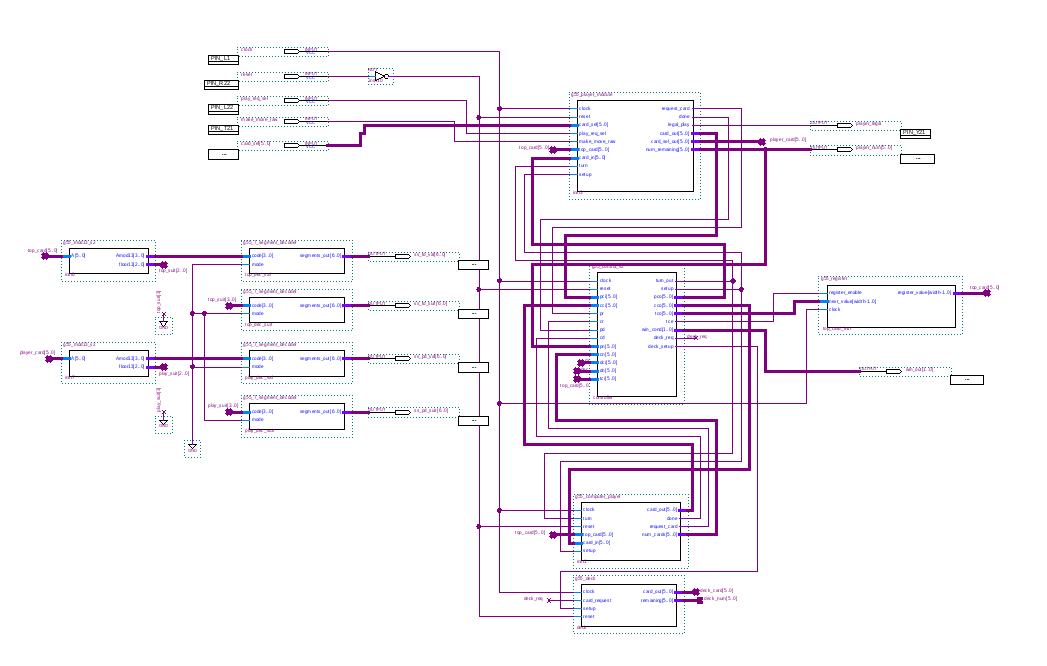
\includegraphics[scale = 0.45, angle=90, origin=c]{graphics/complete-circuit.png}
\caption{\textit{g55\_system\_v2} Schematic}
\end{figure}

\begin{figure}[H]
\centering
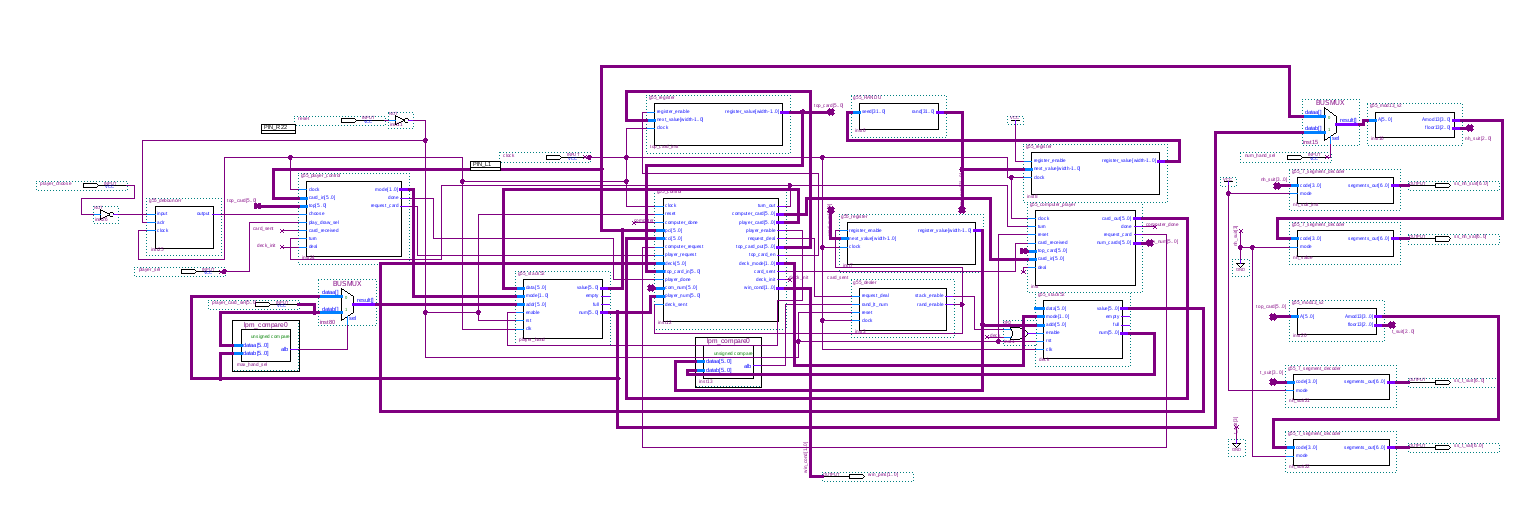
\includegraphics[scale=0.3, angle = 90, origin = c]{graphics/initial-circuit.png}
\caption{\textit{g55\_system} Schematic}
\end{figure}

Two versions of the circuit were made: an initial attempt (\textit{g55\_system} in Figure 2) and a second attempt (\textit{g55\_system\_v2} in Figure 1). In all other sections, \textit{g55\_system} refers to \textit{g55\_system\_v2}, not the first version.

\subsection{Player Module}

\subsection{Computer Player Module}

\subsection{Controller}

\section{Testing}

\section{FPGA Utilization}
The total FPGA utilization without the use of SignalTap II is 2,682 total logic elements (14\%), 2,053 total combinational functions (11\%), 1,078 dedicated logic registers (6\%), 47 used pins (15\%), and 7,488 memory bits (3\%). The $F_{max}$ reported by TimeQuest Timing Analyzer is 39.07 MHz, less than the desired clock speed of 50 MHz. Overall most if not all components have a negative slack, meaning that the time it takes for a signal to propogate is greater than the maximum time for desired operation. This remains true even if the clock speed is reduced to 27 MHz..

\section{Discussion of Results}
The circuit does not operate as desired. While state transitions in \textit{g55\_controller}, \textit{g55\_player\_module}, and \textit{g55\_computer\_player} appear to work, the circuit does not operate correctly from setup. First, the computer player's hand immediately increases to 52 cards rather than 7, while the player's hand only increases to 3. The \textit{g55\_deck}, however, pops the correct number of cards and the controller believes everything went correctly. The displays for the player's selected card always shows 0, and it appears that it selects one card above the highest filled entry in the stack. However the \texttt{player\_legal} signal does update moving through the deck and so it seems that the cards the player does receive are not identical. Operations to get a card from the deck or play a card often end up getting or playing multiple cards respectively. The first card put on top of the play pile is random. \\

It seems that the communication between modules and the exactly state operations of \textit{g55\_computer\_player} are flawed. Words exchanged between modules is done where the receiving module waits for the input to change and the sender is supposed to keep this signal until the next request is made. However this communication frequently fails with multiple actions being taken for a single request and data not properly being sent. The sender should probably confirm that the output data is correct before the receiver begins to use it, and a change in an input is not robust enough to signal a word has been sent. Most of these problems stem from a desire to get as much done in as few clock pulses as possible. As it stands operations that are expected to be completed by a certain time are not and there is not enough time allowed for signals to propagate through the circuit and be operated upon. It would be interesting to see if any paths can be minimized so a signal propagates faster. However the main solution to these problems would come from allowing operations to occur in a longer time frame and ensure that data transferred and received is valid.

\end{document}